
\section{The Moodle Platform}
\label{sec:moodleplatform}
	General about the platform






\subsection{Courses}
	How does courses work.






\subsection{Groups}
	What is groups and groupings and how is it related to courses. Can we use it?




\subsection{Plugin}
	General about plugins: there are lots o them 




	\subsubsection{Blocks}





	\subsubsection{Activity modules}





	\subsubsection{Admin Tools}






	\subsubsection{Local Plugins}




\subsection{Framework}
	Something about forms, pages, filtering and possible more.
	
	
	
	
	
	\subsubsection{Database Layer}
	
	
	
	
	
	\subsubsection{Context System}
	%(http://docs.moodle.org/dev/Roles_and_modules)
	%(http://docs.moodle.org/dev/File:Moodle-contexts-1.8.png
The context system in moodle is used to set the context of a given page to determine the users capabilities and which blocks to present.
 
When a user is logged in to a Moodle system he can have various roles in various contexts. 
One person might be a student in one course and a teacher in others. 
Moodle use a hierarchical context system to manage users roles and their capabilities. 
The context systems hierarchical layout can be seen in figure \ref{fig:moodle-contexts}.
 
 \begin{figure}
	 \centering
		 %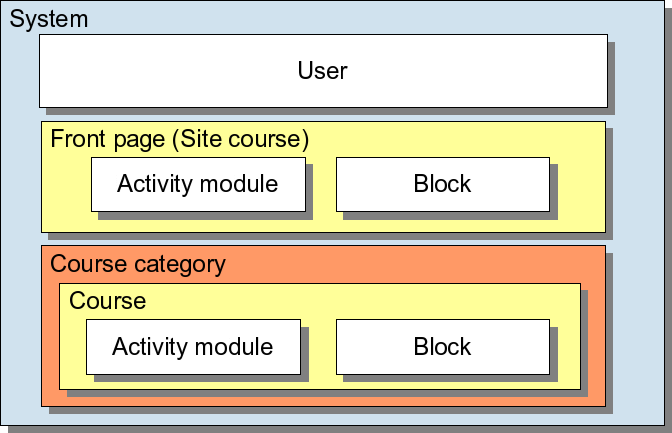
\includegraphics[width=\textwidth]{images/moodle-contexts.png}
	 \label{fig:moodle-contexts}
	\morscaption{The hierarchical context structure in moodle}
 \end{figure}

The highest level of context is the system context which all inherit from. 

Every page in moodle which is loaded directly through HTTP(S) must set the page context. 
An example of how to set the context can be seen in code snippet \ref{courseviewcontextsnippet} from \moodlefile{/course/view.php}, which loads the default page of a Moodle course.

\begin{lstlisting}[style=phpCode, caption=\myCaption{A snippet from \moodlefile{/course/view.php}}, label=courseviewcontextsnippet]
...
if (!$context = get_context_instance(CONTEXT_COURSE, $course->id)) {
  print_error('nocontext');
}
...
if ($switchrole > 0 && confirm_sesskey() &&
  has_capability('moodle/role:switchroles', $context)) {
...	
\end{lstlisting}
The function \fu{get\_context\_instance} requires a constant and in this case a course id. 
In this example an error is outputted if the context fails to load. 
%http://docs.moodle.org/dev/Roles_and_modules#has_capability_.28.24capability.2C_.24contextid.2C_.24kill.29
To determine whether or not an user has the capability to do certain actions the function \fu{has\_capability} is used. It requires a string specifying which capability and the context for the current page. 
It i required to set the context for each page. 
%http://docs.moodle.org/dev/Page_API#Context
In some pages Moodle sets the context itself. 

Beside being responsible for capabilities contexts are usedto determine the presented blocks on a page. If an user with the capability to edit a course page adds a block and the instance is set to the system context the block will be showed on all course pages. If the context is set to the course context the block will only be presented on that courses page. 

	
	
	